\section{Hours of Operation and Occupancy}
\label{sec:hoo}

\subsection{Hours of Operation}
\subsubsection{Overview}
Hours of operation are added to the model using operation start time and duration inputs. The start times and durations are assigned to each model through the sampling process using a set of distributions based on building type. They are then further broken down by weekday and weekend (Figure~\ref{fig:start_time} and Figure~\ref{fig:duration}). When applied to the model, the start time and duration are used to establish operating hour start and end times. These times are used to adjust the other schedules in the model (e.g., lighting, thermostat). This is achieved by stretching or shrinking the schedule on the temporal axis to align all schedules with the operating hours for the model. Note that because the weekday and weekend start times and durations are sampled independently, they are not aligned in a given building model.

\subsubsection{Hours of Operation Derivation}
We derived the hours of operation by applying the method introduced in \cite{bianchi2020modeling} to 1 year of AMI data from 6,070 buildings spread across eight utilities (the commercial schedules AMI data set). We first extracted the two-dimensional distribution of \textit{High Load Start Time} and \textit{High Load Duration} from this AMI data set, as an approximation of the schedule of hours of operations for each building type. Then, we compared this distribution with the inputs of ComStock at the start of
 the \href{https://www.nrel.gov/buildings/end-use-load-profiles.html}{End-Use Load Profiles} (EULP) calibration.

Figure~\ref{fig:utility_building_type} lists the number of buildings for each building type from each utility's AMI data set that was considered during the EULP project. The utility data sets and names are listed in Table 10 of the EULP Final Technical Report \citep{eulp_final_report}. Among the 15 building types considered in ComStock, 14 can be found in the commercial schedules AMI data set. The only exception is secondary schools, because all schools were grouped together in the AMI data.

We compared the distribution extracted from the commercial schedules AMI data set with the inputs of ComStock at the start of the EULP calibration. The results of the small office building type are presented in Figure~\ref{fig:small_office_season} to illustrate the process, because this building type has the largest sample size in the AMI data set. We considered two day types, working day vs. non-working day, and two season definitions---one defined by month, and the other defined by daily average outdoor air temperature. The distribution of hours of operation is more diffuse in the AMI data set than in the ComStock inputs at the start of EULP calibration. Also, the duration of high load is smaller in the real AMI data than in the previous ComStock assumptions.

We explored whether and how the hours of operation are influenced by season (in Figure~\ref{fig:small_office_season}) and by utility (in Figure \ref{fig:small_office_utility}). Some differences can be observed; however, due to the modeling complexity and the desire to create a nationally applicable approach that avoids overfitting to a specific utility region, we combined the AMI data across seasons and utilities to generate a distribution of hours of operation for each building type. These new distributions were applied to ComStock in place of the existing distributions.


\subsection{Occupancy}
\subsubsection{Occupancy Density}
Occupants are assigned to individual space types as an occupancy density (people/1000 ft\textsuperscript{2}). This value, when multiplied by the total zone floor area, determines the maximum number of people in a zone.  \Crefrange{tab:food_service_occupancy_density}{tab:warehouse_occupancy_density} show the occupancy densities for all space types included in ComStock.

The majority of the ComStock occupancy density values are from the DOE prototype models. These are derived primarily from ASHRAE 62.1-2004 \citep{ashrae_62.1_2004}, with some space type densities originating from the International Building Code 2003 \citep{icc_2003}. Prototype hotel guest rooms were assumed to have 1.5 occupants each, and occupancy rates for the two hotel models were assumed to be 65\% to align with the industry average occupancy rate and \cite{jiang_2008}. Rooms were randomly assigned occupants so that 65\% of the rooms were occupied. Most of the DOE prototype hospital and outpatient space type occupancy densities were replaced with values from the 2007 Green Guide for Healthcare (GGHC), which includes typical occupancy densities for healthcare space types \citep{gghc_2007}.

\subsubsection{Occupancy Schedules}
The maximum number of people in a zone (calculated from occupancy density and zone floor area) is multiplied by an hourly occupancy schedule with values ranging from zero to one to capture the variation in building occupancy throughout the day. Figures \ref{fig:occupancy_schedules_1} and \ref{fig:occupancy_schedules_2} show the national base occupancy schedules used in ComStock, broken down by building type. For the California occupancy schedules, please see figures \ref{fig:occupancy_schedules_deer_1} and \ref{fig:occupancy_schedules_deer_2} in the Appendix. For buildings in all states except California, the base schedules are the DOE prototype occupancy schedules. California uses schedules from DEER prototype models \citep{cpuc_deer}. The DOE prototype documentation \citep{deru_2011} notes that there are few data sources that provide operating schedules for use in building energy simulations. Thus, the schedules in the prototype models were derived from two primary data sources: the Advanced Energy Design Guide Technical Support Documents \citep{jiang_2008,doebber_2009,liu_2007,pless_2007} and ASHRAE 90.1-1989 Section 13 \citep{ashrae_1989}. These schedules were then modified to account for real-world building operation, based on the experience of the engineers who created the DOE prototype models. Classroom occupancy schedules for primary and secondary schools were adjusted by factors of 0.75 and 0.70, respectively, to meet the student numbers documented in \cite{pless_2007}. Table~\ref{tab:occupancy_schedule_source} lists the data sources for occupancy schedules in each of the prototype buildings (both DOE and DEER). Occupancy schedules in ComStock buildings are further adjusted so that the total daily occupancy in the building stock does not exceed the average daily occupancy of the United Stated building stock as derived from analysis of locations in the American Time Use Survey \citep{atus2018} Activity file. This adjustment applies a 23\% reduction factor to all occupant schedule values, resulting in a peak daily total occupancy in ComStock models of approximatly 115M people.

These base occupancy schedules are stretched, compressed, or shifted in time to reflect the model’s assigned hours of operation. For example, the base occupancy schedule for large offices is 9 a.m.--5 p.m. (8 hours of operation). If one large office model is assigned a start time of 8 a.m. and an operating duration of 10 hours, the base schedules in the model will be stretched so that the occupied period is an additional two hours long. All schedules in the model (occupancy, lighting, thermostat, plug load, etc.) are modified in the same manner to ensure coordination between occupancy, lighting, etc.


\subsubsection{Occupancy Activity Schedules}
Occupancy activity schedules represent the total heat gain per person, including convective, radiant, and latent heat. An internal EnergyPlus algorithm determines the fraction of the total load that is sensible and latent. The sensible portion is further divided into radiant and convective using the default fraction radiant value. DOE prototype activity levels are fixed for a given building type and range from 120--132 watts per person across the various building types. DEER prototype activity levels vary by space type and range from 117--331 watts per person. Table~\ref{tab:activity_schedule} lists the occupancy activity schedules used in ComStock.

\pagebreak

\begin{figure}
   \centering 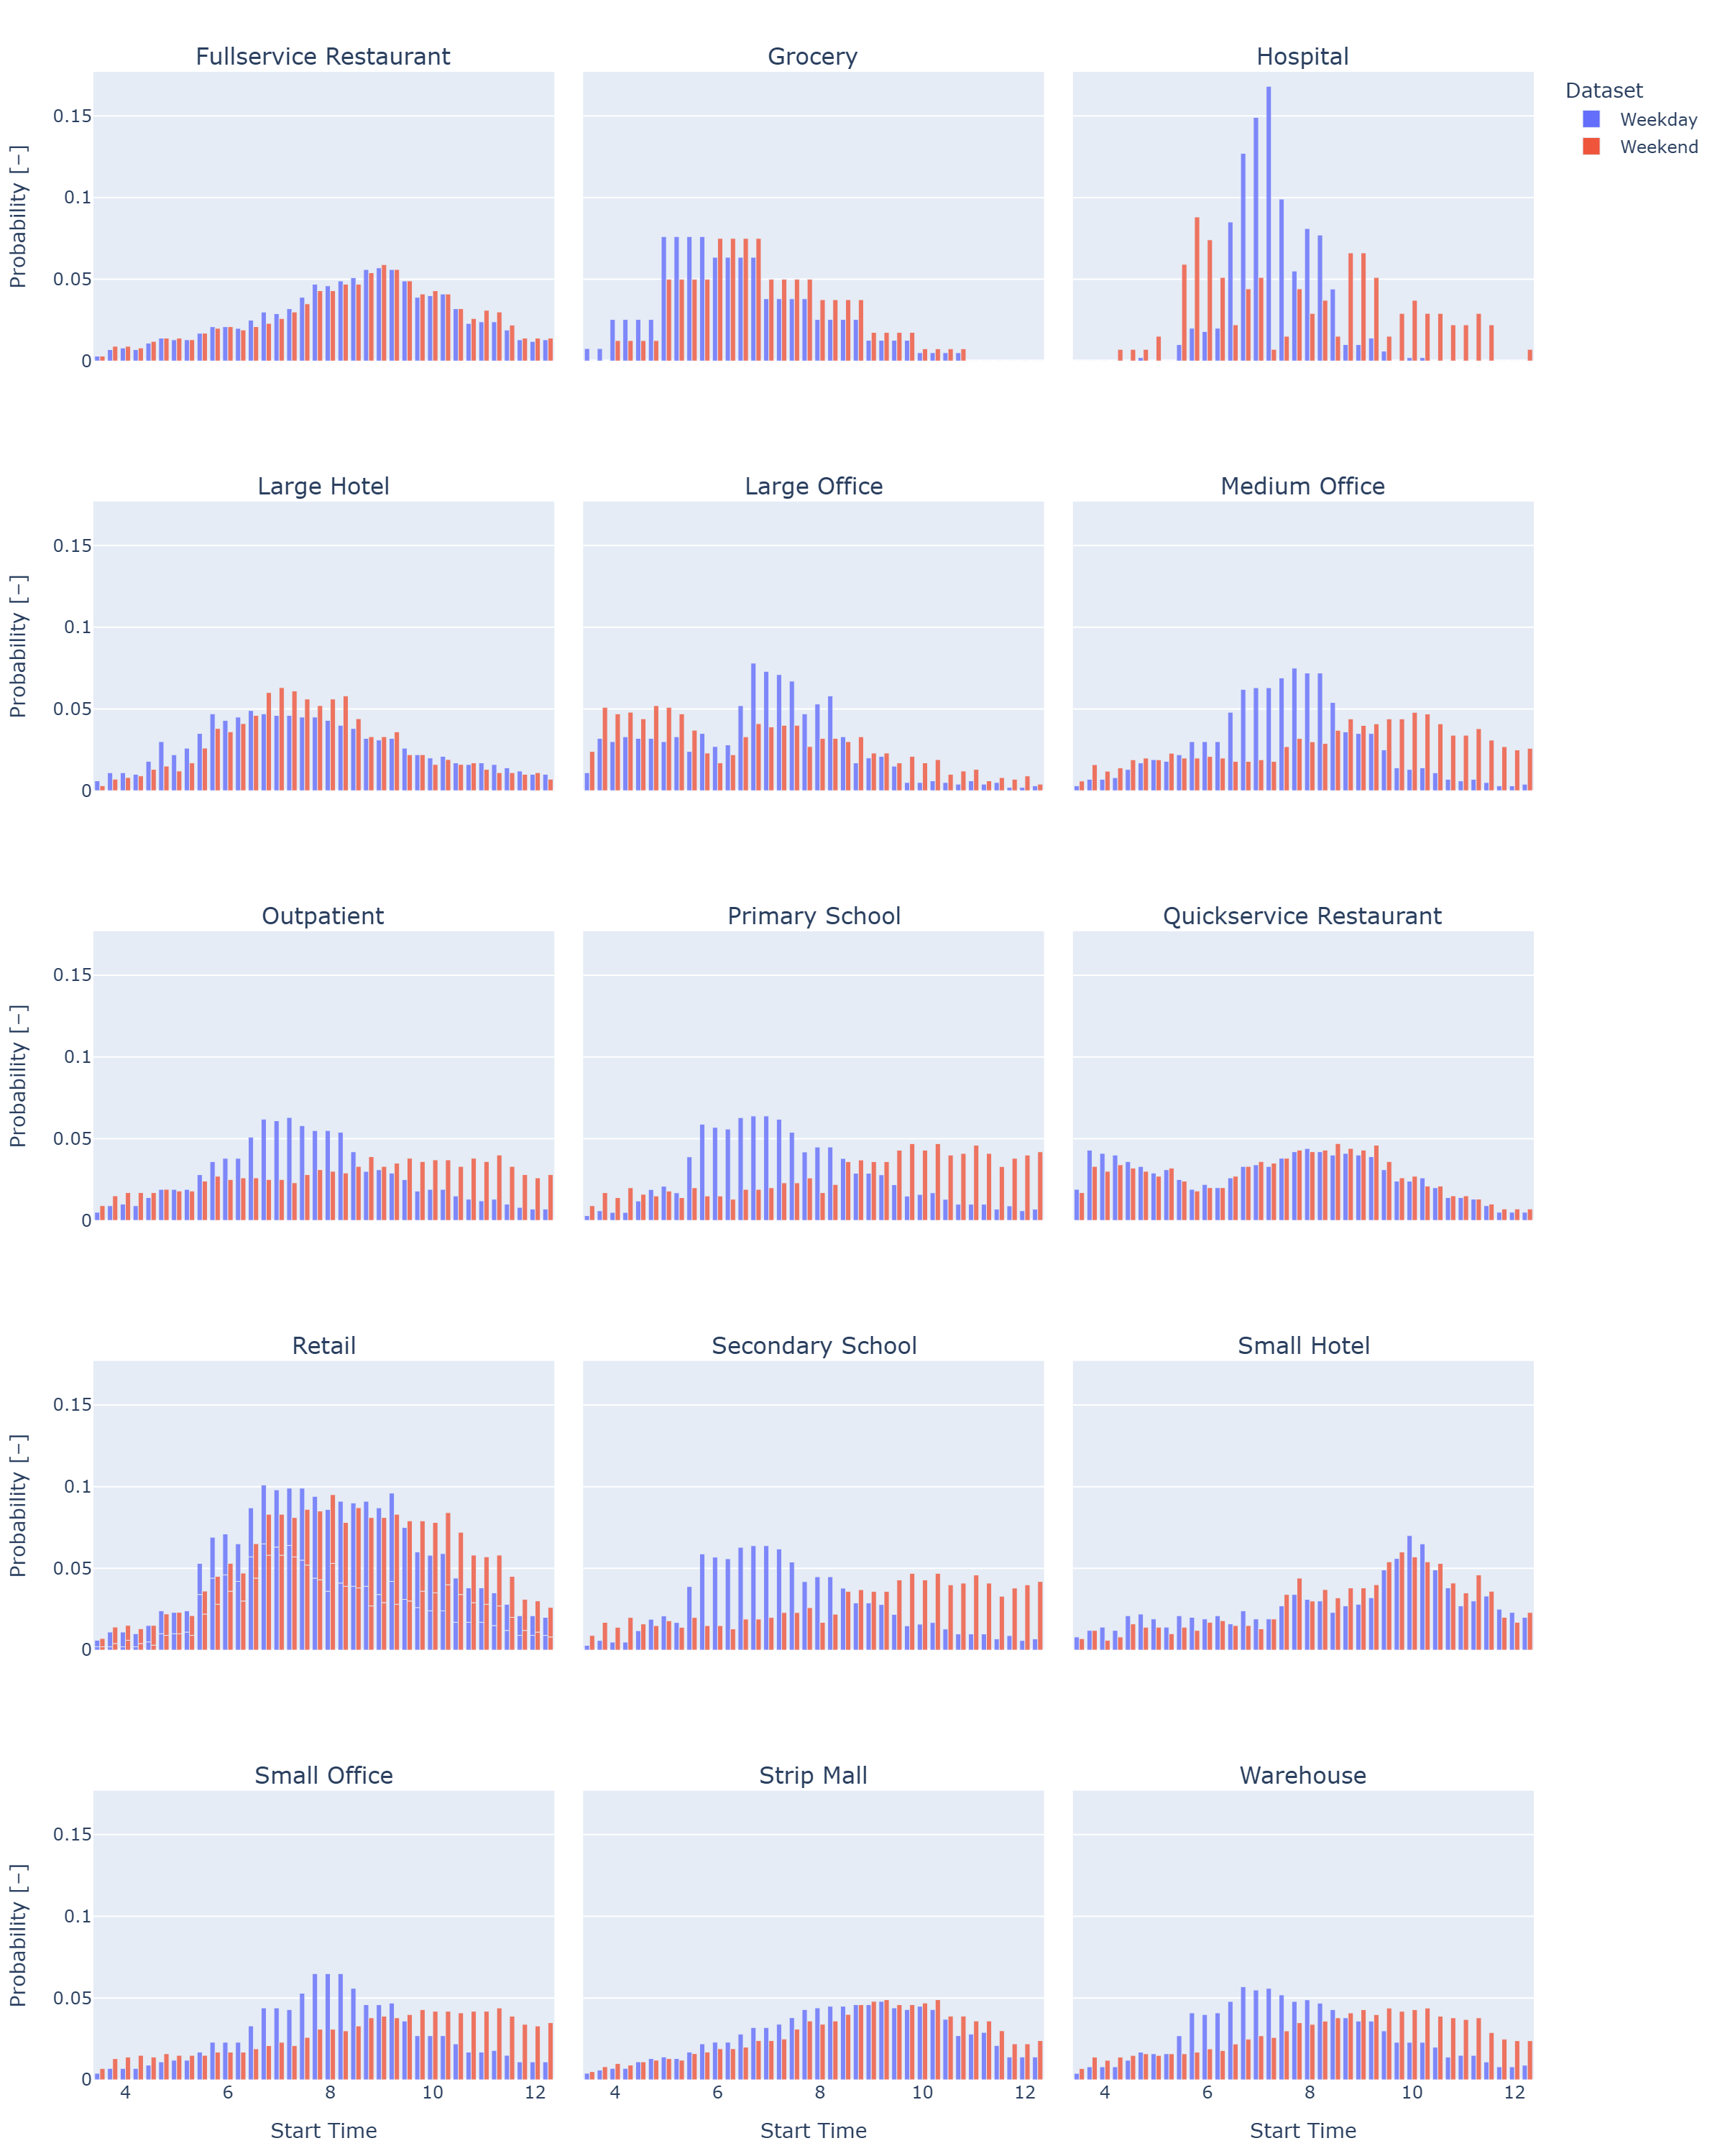
\includegraphics[width=1\textwidth]{figures/start_time.png}
   \caption{Operating hours' start time distributions.}
    \label{fig:start_time}
\end{figure}

\begin{figure}
    \centering 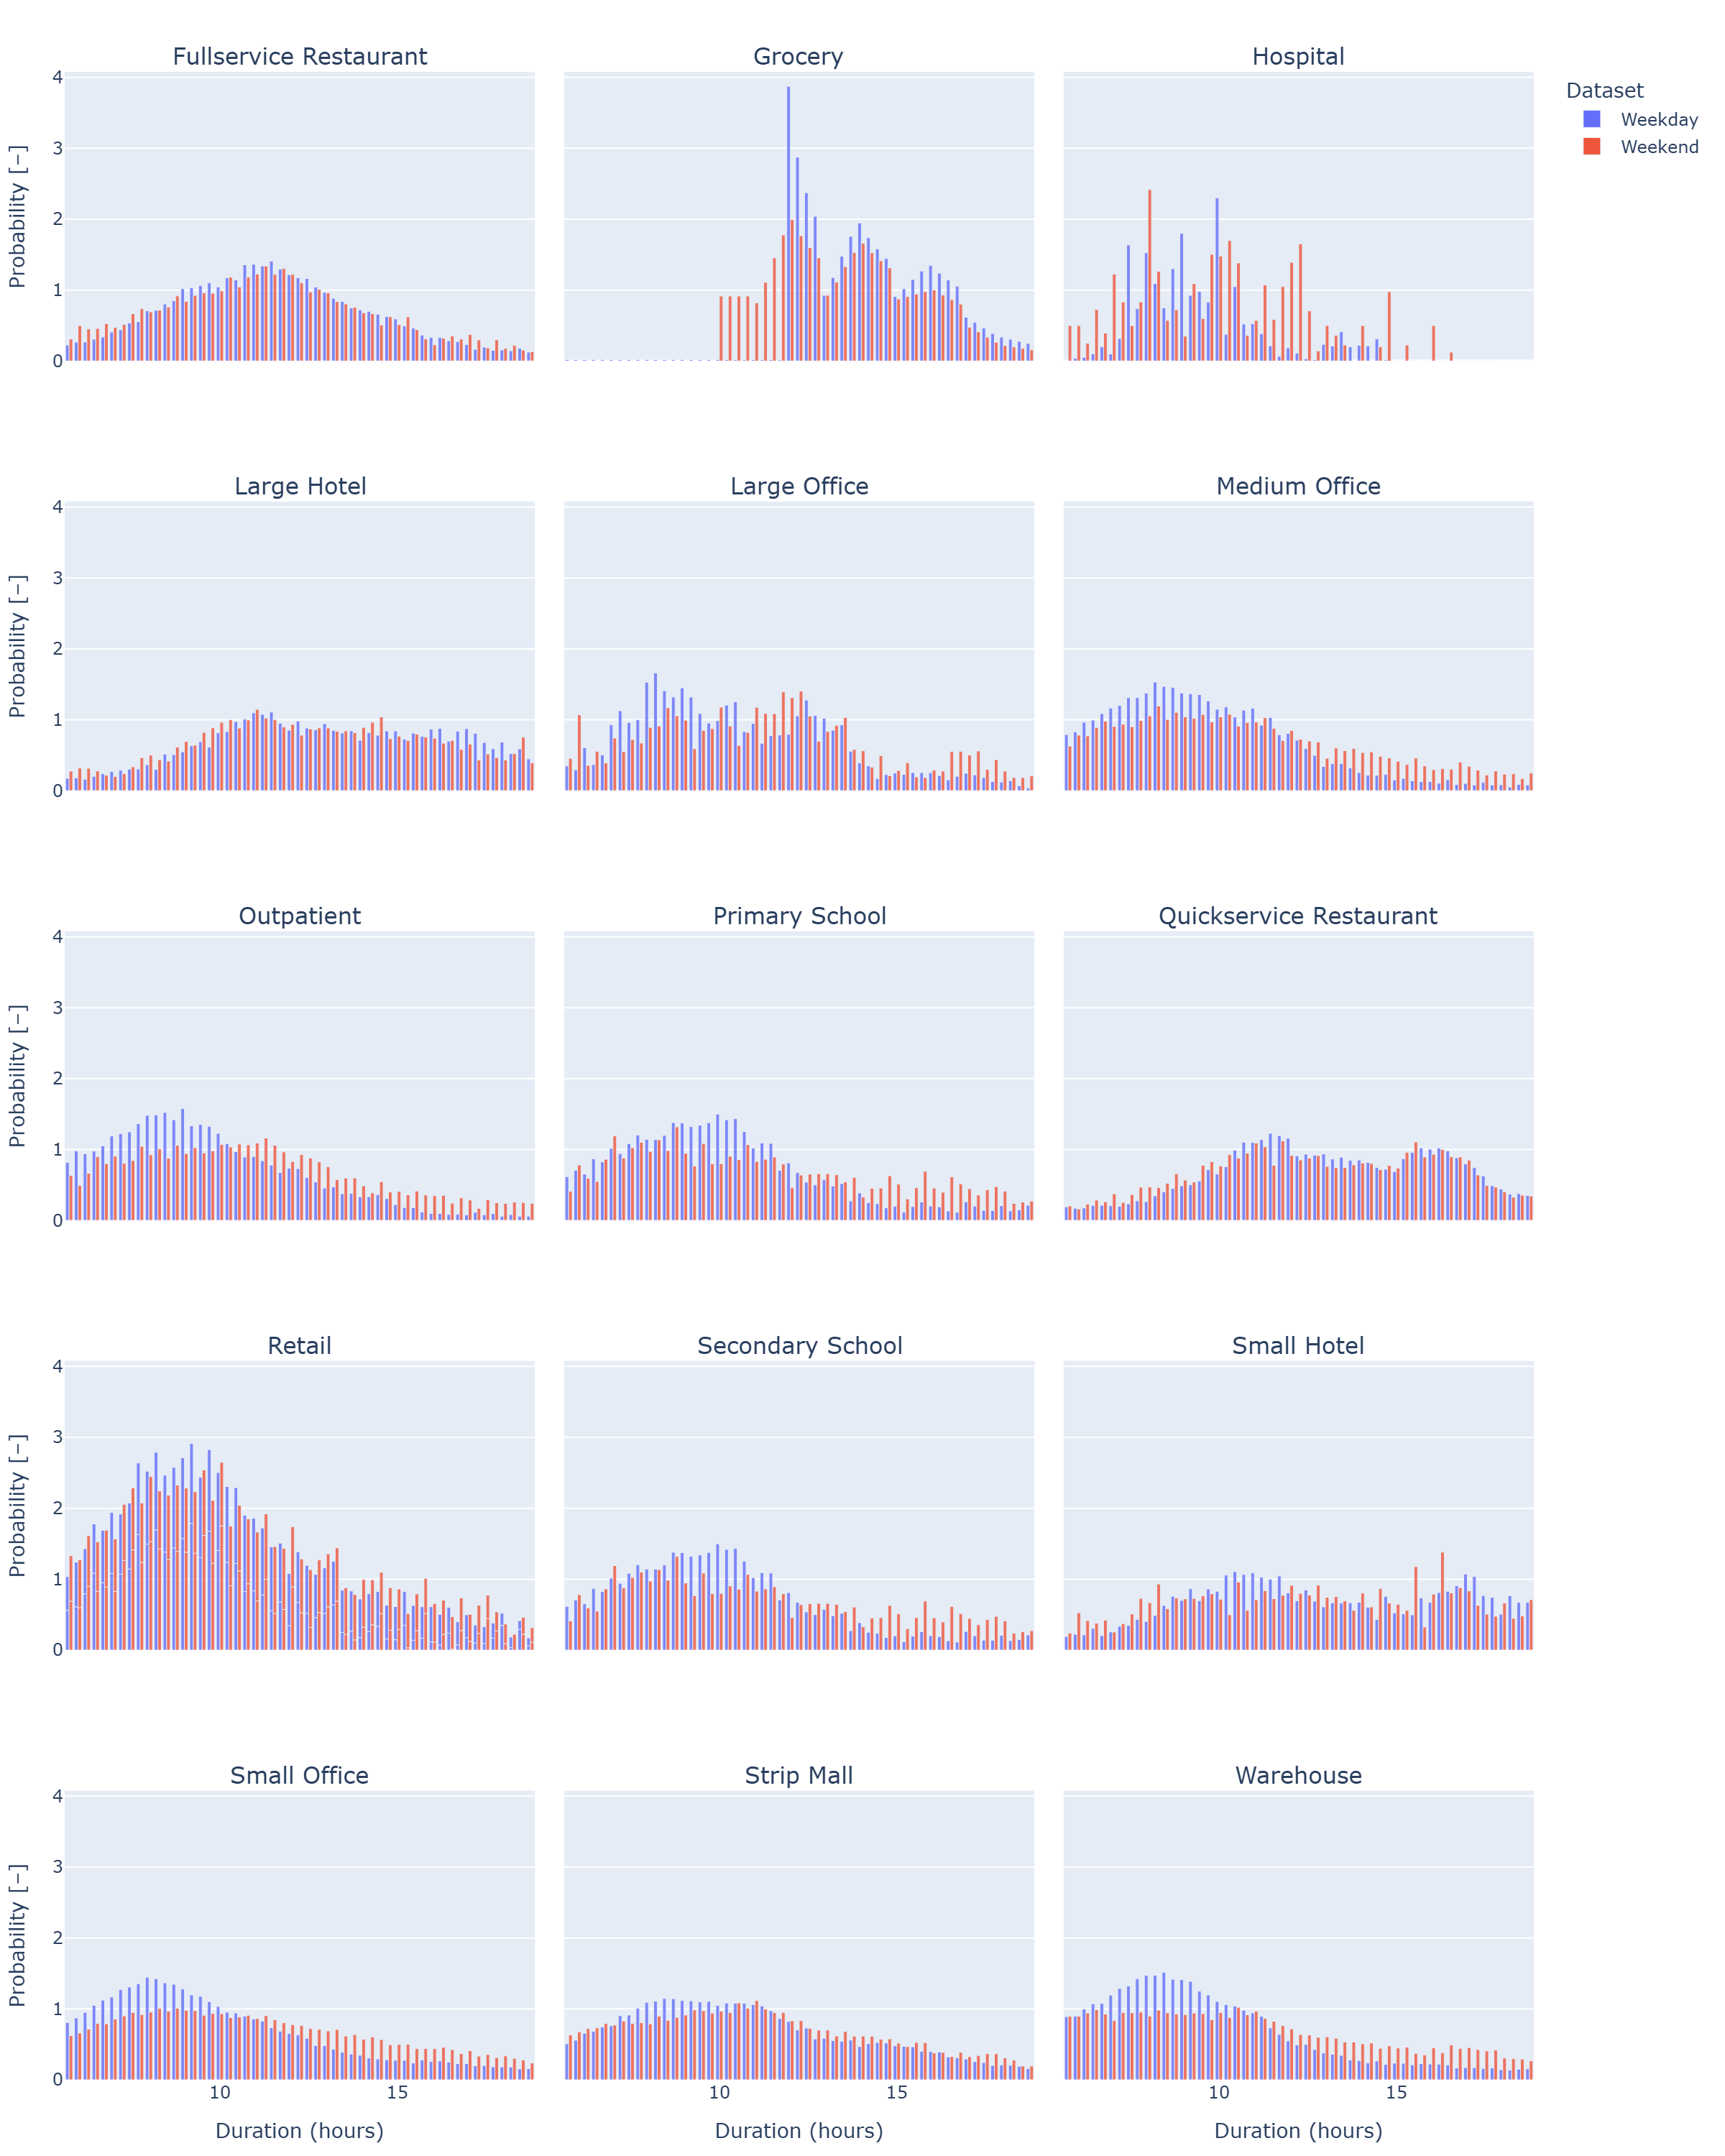
\includegraphics[width=1\textwidth]{figures/duration.png}
    \caption{Operating hours' duration distributions.}
    \label{fig:duration}
\end{figure}

\begin{figure}
    \centering 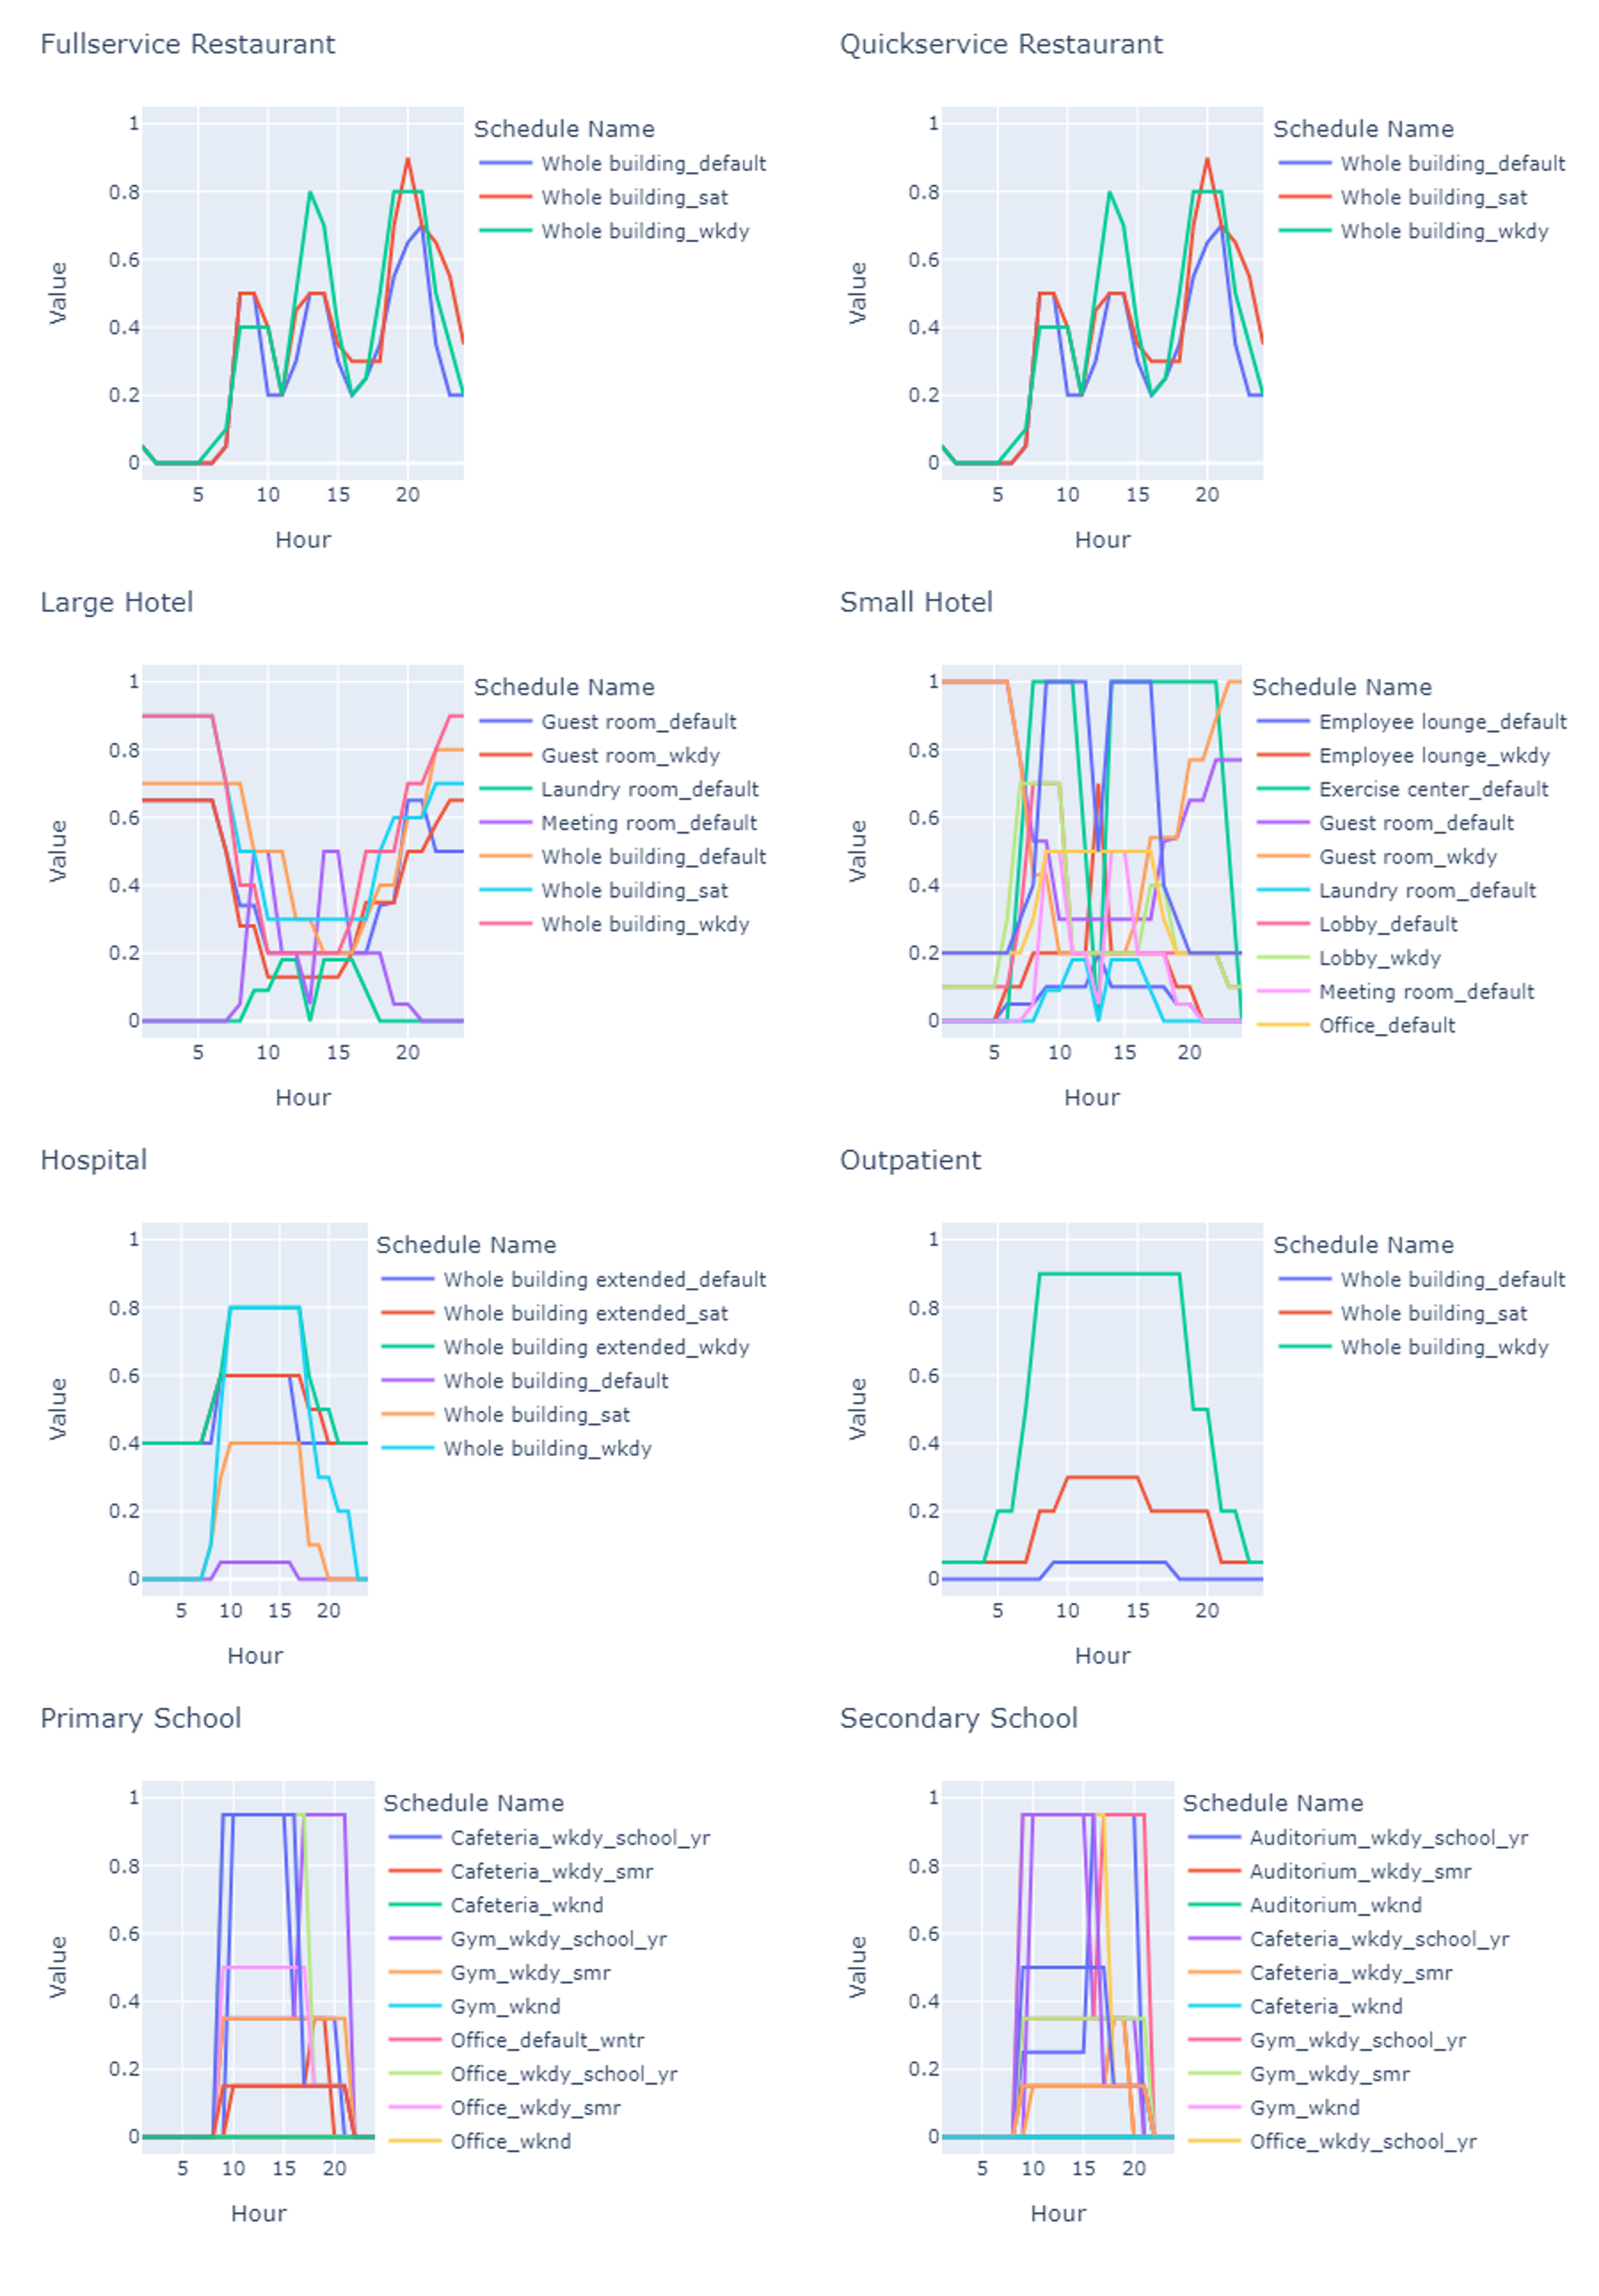
\includegraphics[trim={0 0 0 0}, clip,  % L B R T
    width=0.9\textwidth]{figures/occupancy_schedules_1.png}
    \caption[National base occupancy schedules excluding California]{National base occupancy schedules for food service, lodging, healthcare, and education ComStock building types, excluding California. See Figure \ref{fig:occupancy_schedules_deer_1} for California.}
    \label{fig:occupancy_schedules_1}
\end{figure}

\begin{figure}
    \centering 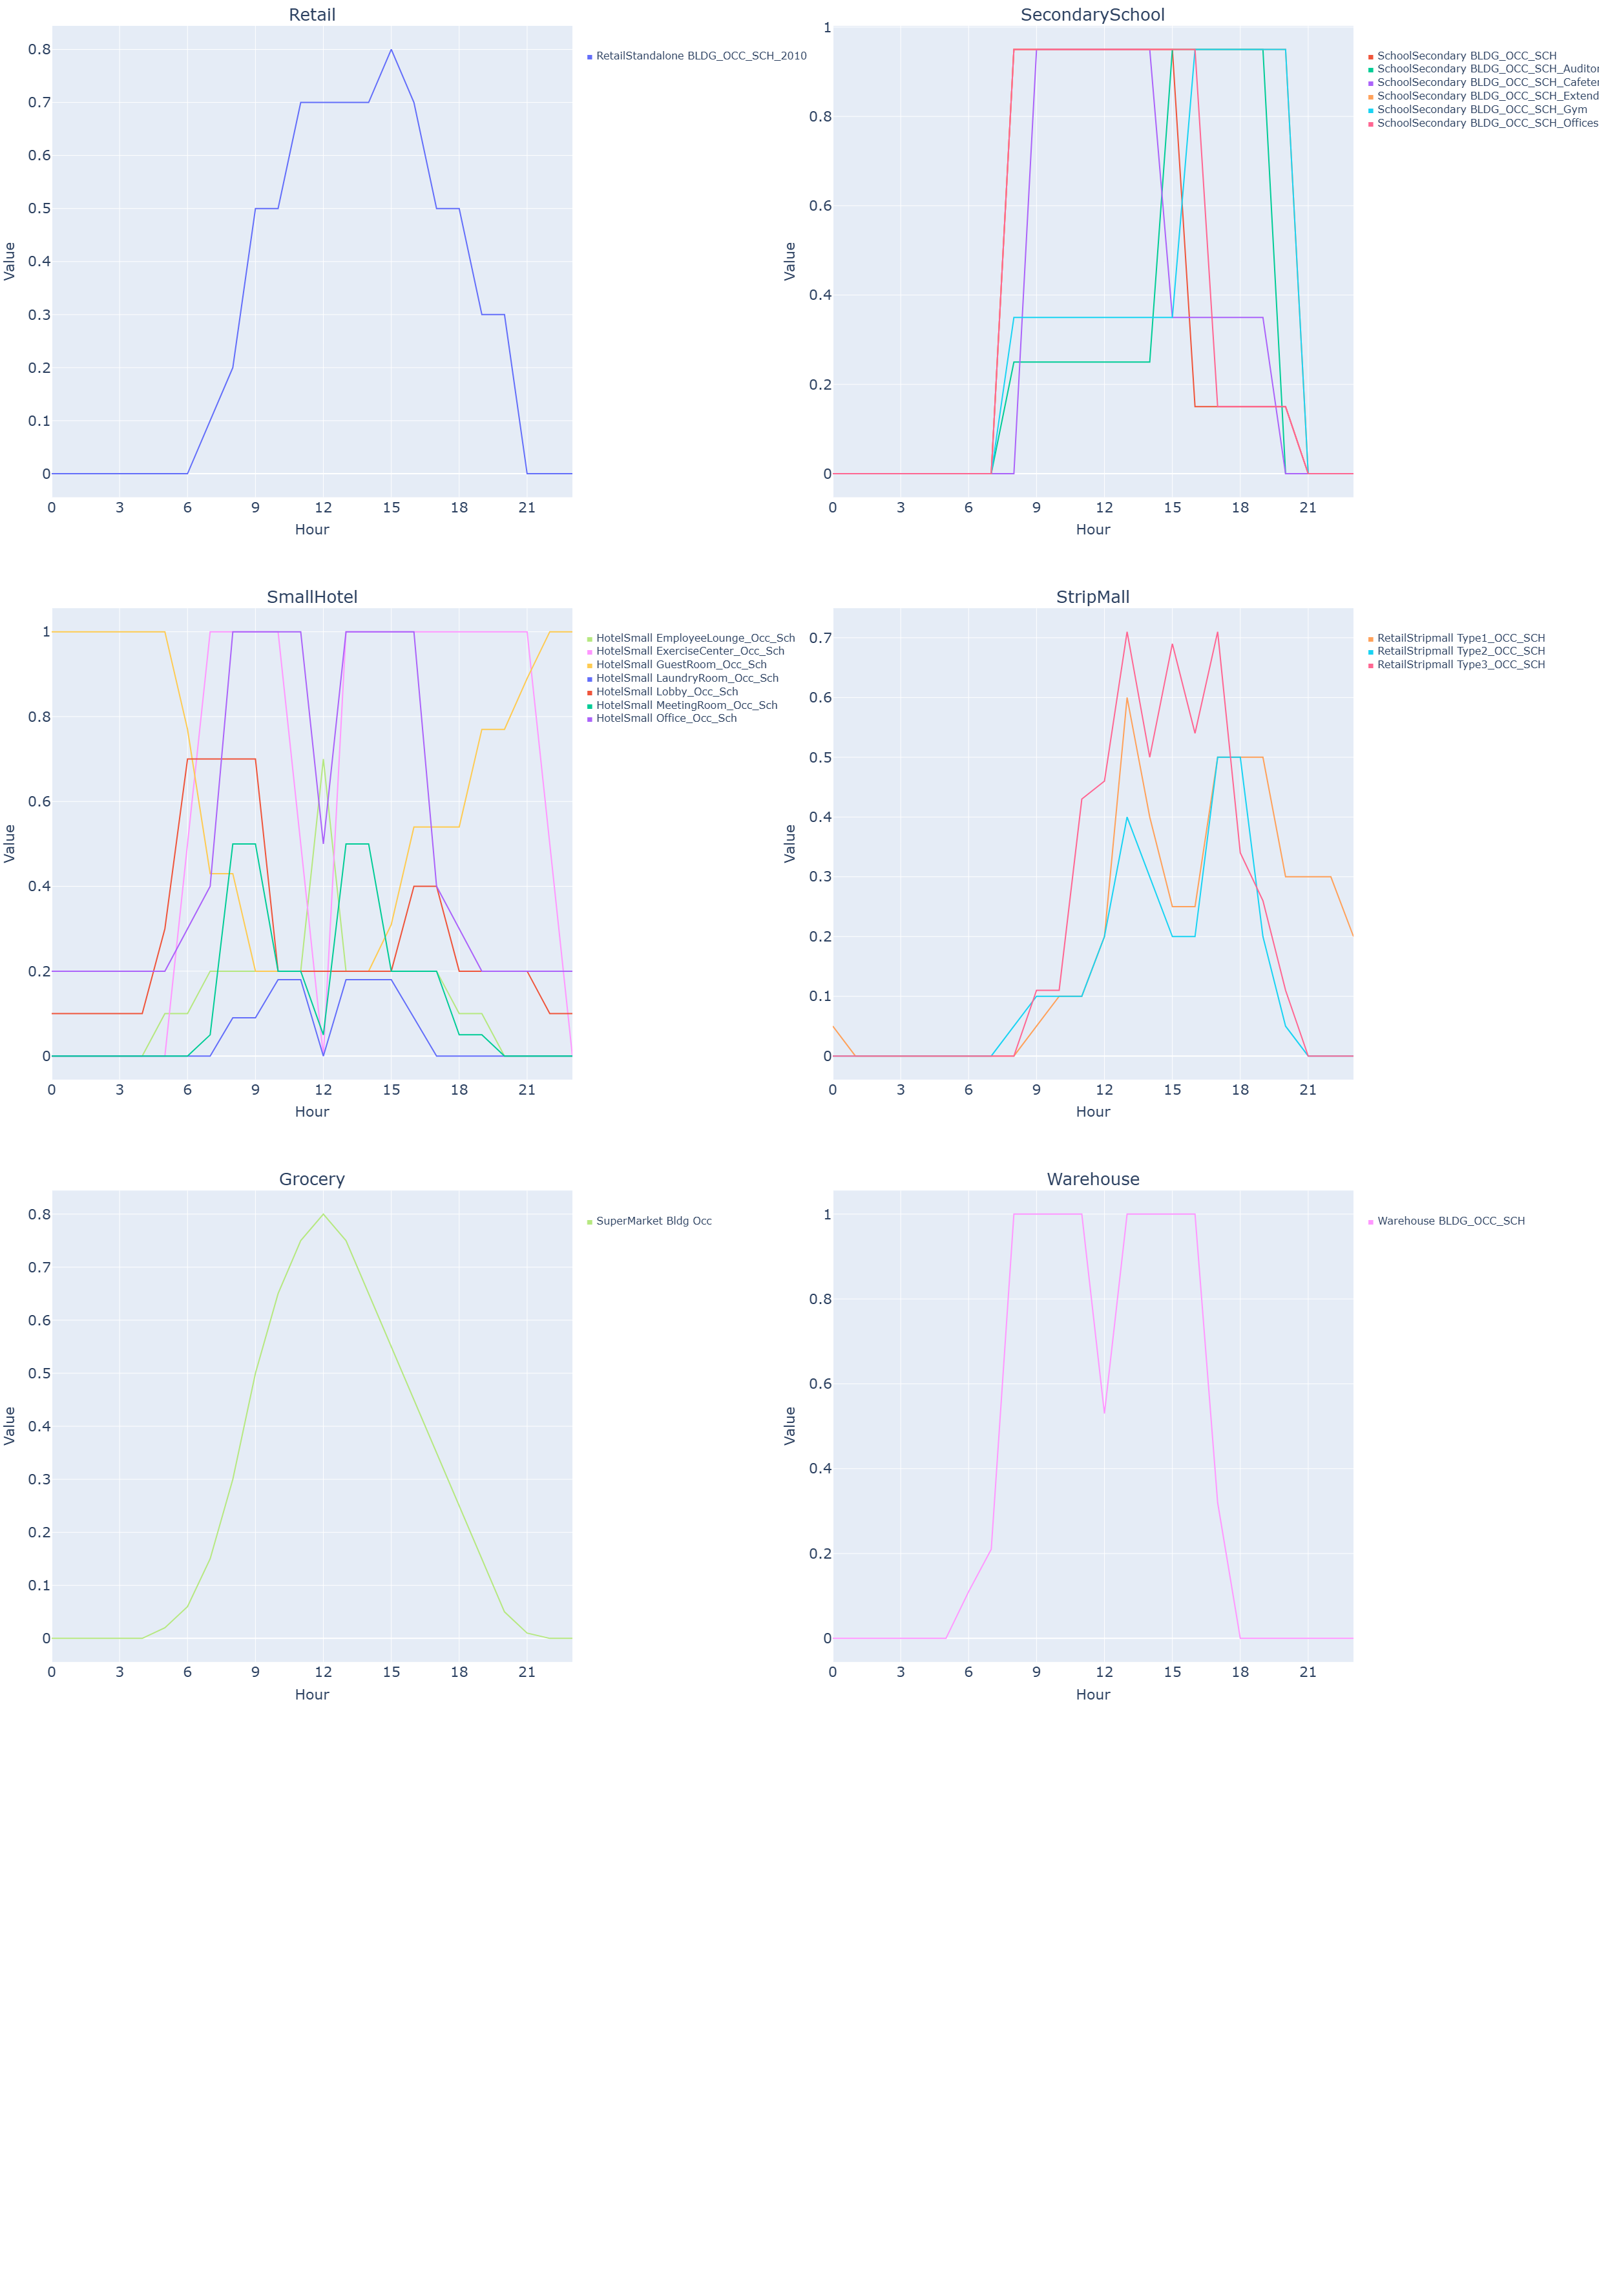
\includegraphics[trim={0 0 0 0}, clip,  % L B R T
    width=0.9\textwidth]{figures/occupancy_schedules_2.png}
    \caption[National base occupancy schedules excluding California]{National base occupancy schedules for retail, office, and warehouse ComStock building types, excluding California. See Figure \ref{fig:occupancy_schedules_deer_2} for California.}
    \label{fig:occupancy_schedules_2}
\end{figure}